\documentclass[tikz,border=5pt]{standalone}

\usepackage{tikz}

\begin{document}

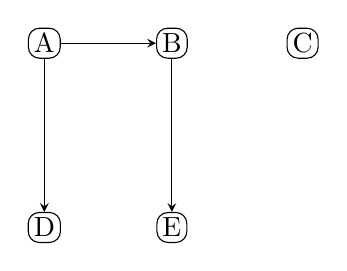
\begin{tikzpicture}[
  canon node/.style={draw, rounded corners, inner sep=2pt},
  canon edge/.style={->, >=stealth}
]
\node[canon node] (A) at (2.50, -2.68) {A};
\node[canon node] (B) at (4.12, -2.68) {B};
\node[canon node] (C) at (5.78, -2.68) {C};
\node[canon node] (D) at (2.50, -5.02) {D};
\node[canon node] (E) at (4.12, -5.02) {E};
\draw[canon edge] (A) -- (B);
\draw[canon edge] (A) -- (D);
\draw[canon edge] (B) -- (E);
\end{tikzpicture}

\end{document}
